\documentclass{MScthesisITEM}

% this package is just to generate text for demo-purposes
\usepackage{blindtext}
\title{POSITION CONTROL FOR AUTOMATIC LANDING OF UAV IN A NET ON SHIP} % The title of your assignement; NB use \newlinetitle to start a newline
\author{Kjetil Hope Sørbø} % Your firstname and lastname
\professor{Thor Inge Fossen, Tor Arne Johansen} % Affiliation = ITEM for instance
%\supervisor{Firstname Lastname, Affiliation}

%% Uncomment the following in case you want subfigures; note that there will be a warning for the caption package
 \let\subcaption\undefined
 \let\subfloat\undefined
 \usepackage[bf]{caption}
 \usepackage{subcaption}





\providecommand{\keywords}[1]{\textbf{\textit{Keywords:}} #1}

\DeclareGraphicsExtensions{.pdf,.jpg}
\graphicspath{{./figs/}}

\loadglsentries{glossary}
\makeglossaries


\begin{document}


\selectlanguage{english}
\pagenumbering{roman}
\pagestyle{plain}

%% Only for the project; comment out the line below for the master's thesis; the front page will be generated automatically by DAIM
\titleITEM

%% Only for the master's thesis; for the project report the description is taken from It's Learning and added by the department
% \selectlanguage{english} % Change to 'norsk' if you are writing in Norwegian
% \begin{titlingpage}

\noindent
\begin{tabular}{@{}p{4cm}l}
\textbf{Title:} 	& \thetitle \\
\textbf{Student:}	& \theauthor \\
\end{tabular}

\vspace{4ex}
\noindent\textbf{Problem description:}
\vspace{2ex}

\noindent \Blindtext[2][1]
\vspace{6ex}

\noindent
\begin{tabular}{@{}p{4cm}l}
\textbf{Responsible professor:} 	& \theprofessor \\
\textbf{Supervisor:}			& \thesupervisor \\
\end{tabular}

\end{titlingpage}
% \cleardoublepage

%% There must be an abstract in English, even though the main text is in Norwegian
\selectlanguage{english}
\pagestyle{empty}
\begin{abstract}
%Automatic landing of a fixed wing \acrfull{uav} in a net on a ship require an accurate positioning system. There exist today high-end systems with such capability for special applications, e.g military systems and costly commercial systems, which restrict the availability of such systems. To increase the general availability these systems must consist of low-cost components. Here, an alternative is the use of low-cost \gls{gnss} receivers and apply \gls{rtk-gps}, which can provide centimeter level position accuracy. However the processing time for the \gls{rtk-gps} system results in degraded accuracy when exposed to highly dynamical behaviour.
%
%This work present two alternative software and hardware position systems suitable for use in navigation system which apply \gls{rtk-gps}, namely \gls{rtklib} with a Ublox Lea M8T receiver and a Piksi system. Both the Piksi and the Ublox receiver are single-frequency \gls{gnss} receivers. These systems will in this work be compared and their individual capability to provide accurate position estimate will be evaluated. 
%
%The \gls{rtk-gps} system is implemented in DUNE (DUNE:Unified Navigation Environment) framework running on an embedded payload computer on-board an \gls{uav}.
%
%The performance of these position systems are in this work investigated by experimental testing. The testing showed that the \gls{rtklib} performed better than the Piski alternative, and further showed the tested navigation system provide sufficient quality for integration into a control and guidance system, allowing for automatic landing of an \gls{uav} in a net.

\end{abstract}
%\keywords{UAV,RTK-GPS,}

\cleardoublepage

%% Only for the master's thesis; if the main text is in English and you can write Norwegian, there must be an abstract in Norwegian as well.
% \selectlanguage{norsk}
% \pagestyle{empty}
\renewcommand{\abstractname}{Sammendrag}
\begin{abstract}
\noindent Denne avhandlingen presenterer ett bane- og navigasjonssystem, som brukes i et autonomt nett landingssystem for en fast-vinge \acrfull{uav}. Landingsbanen til en \gls{uav} kan konstrueres som en rett linjet bane, men for at en \gls{uav} skal kunne følge landingsbanen må \gls{uav}en være i en posisjon hvor det finnes en mulig bane til landingsbanens start posisjon. Dette motiverer utviklingen av en innflyvingsbane logikk mot landingsbanen sin inngangs posisjon fra hvilken som helst innledende startposisjon i luftrommet.

I tillegg til et bane genererende system trenger \gls{uav}en ett robust høy nøyaktighets navigasjonssystem. Dette gjøres med å bruke \acrfull{rtk-gnss}, som kan gi centimeter nøyaktighet. En ulempe med \gls{rtk-gnss} er at det kan miste lås på satellitter som fører til tap av funksjonalitet. I dette arbeidet kompenseres dette ved å benytte et sekundært \acrfull{gnss} system. For å håndtere tap av \gls{rtk-gnss} er et robust \gls{rtk-gnss} system foreslått, hvor tidligere gyldige \gls{rtk-gnss} posisjon løsninger er kombinert med det sekundære \gls{gnss} systemet, for å bli brukt til å kompensere det eksterne navigasjon systemet. Denne kompensatoren er utformet slik at det eksterne navigasjonssystemet får samme nøyaktighets nivå som \gls{rtk-gnss} i en kort periode, inntil enten \gls{rtk-gnss} kommer tilbake eller blir frakoblet. Med denne kompensatoren blir navigasjonssystemet til \gls{uav}en robust mot korte tap av \gls{rtk-gnss}, og tilgjengeligheten til \gls{rtk-gnss} er utvidet.

Både eksperimentell testing og \acrfull{sil} verifikasjon har blitt utført for å teste \gls{uav}ens evne til å lande i et stasjonært nett plassert på en tilfeldig posisjon. For å bedre navigasjon og ytelse, har en mobil sensor enhet blitt benyttet for å få posisjonen til nettet. Denne sensoren enheten ble benyttet under testing, hvor den viste seg å gi det tiltenkte bidraget.
\end{abstract}
% \cleardoublepage

\selectlanguage{english}% Change to 'norsk' if you are writing in Norwegian

%\renewcommand{\abstractname}{Preface}
\begin{abstract}
\noindent This thesis is submitted in partial fulfillment of the requirements for the Master of Science degree at the Norwegian University of Science and Technology.

The work presented in this thesis has been carried out at the Department of Engineering Cybernetics, and would not have been possible without the inputs and contributions from many of its associates. First, I would like to thank Professor Tor Arne Johansen and Professor Thor Inge Fossen for their inspiring ideas and guidance into the academic world. A huge thanks goes to Kristian Klausen for his invaluable help and guidance at the UAV-Lab. Furthermore I want to thank the UAV-pilots Lars Semb and Pål Kvaløy for excellent flying. I would also like to thank my fellow MSc. students at the UAV-Lab. They gave me invaluable feedback and made a coordinated development of the autonomous landing system possible.

Finally I want to thank my parents and brothers for their never-ending support and guidance.
\begin{center}
\emph{Trondheim, June, 2016} \\
\emph{Kjetil Hope Sørbø}
\end{center}
\end{abstract}
%\cleardoublepage

% similarly you may add a separate acknowledgments page

\tableofcontents*
\cleardoublepage

%% include if relevant
%\listoffigures
%\cleardoublepage
%
%%% include if relevant
%\listoftables
%\cleardoublepage

%% include if relevant
%\listofalgorithms
%\addcontentsline{toc}{chapter}{List of Algorithms}
%\cleardoublepage

%% include if relevant
%\printglossary[title=List of Symbols, style=long]
%\cleardoublepage
\glsaddall[]

%% include if relevant
\printglossary[title=Acronyms,type=\acronymtype] % prints just the list of acronyms


\cleardoublepage



\pagenumbering{arabic}
\pagestyle{ruled}
%===================================== CHAP 1 =================================
\chapter{Introduction}
\section{Background}
Recent development of flying \glspl{uav} has been recognized to provide an attractive alternative to work previously performed by manned operations. Typical work which has attracted attention includes inspection, aerial photography, environmental surveillance and search and rescue. Today \gls{uav} operation are becoming more autonomous, however in order to become fully autonomous a fixed wing \gls{uav} must be able to perform a autonomous landing.

An important premise for successful and safe \gls{uav} operation, is the provision of a robust system for safe landing of the \gls{uav} following completed operations. A autonomous landing system require a path generation system that can create a flyable landing path during flight operation from any initial position. In addition the navigation system must have centimeter level accuracy in order for the \gls{uav} to perform a autonomous landing in a net. However with a accurate navigation system the case of what to do when the positioning system degenerates must be resolved such that system failure does not occur. An other premise is that the position of the net is known, and available for the path system. With a known position of the landing net the \gls{uav} must gracefully perform a graceful decent, preferable a glide slope towards the landing net position. The length of the glide slope will be limited by the operator, which dictates that the \gls{uav} must be in the correct pose before starting the decent.
\section{Literature review}
There has been perform several studies on autonomous landing system, and there currently exist commercial available system. However these are typical expensive, and mostly focused on either military or air traffic industry. An available system for \glspl{uav} is the SkyHook that apply INS/\gls{gps}\citep{SkyHook}, however this system require expensive equipment and is limited to a few \gls{uav} systems. The limitation on type of \gls{uav} and high cost restricts the usage of the recovery system, and motivates the research of a low cost recovery system for fixed wing \gls{uav}.

Studies that has been performed on autonomous landing has mostly focused on vision-based guidance, due to previously limited accuracy in low-cost \gls{gnss} receiver system, which is typically single frequency receivers. In the paper \citep{barber2007autonomous} a landing system was proposed that compared the use of barometric pressure measurement and optic-flow measurement for estimation of height above ground. The landing path composed of a spiral path down to a given altitude where a glide slope was used to guide the MAV down to the landing area. The papers showed that optic-flow measurement reduced the average landing error with several meters, however the technique used to guided the \gls{uav} is not suitable for precision landing due to large average error from target. A low cost recovery system for fixed wing \gls{uav} is proposed in the paper \citep{kim2013fully}, where computer vision is used to find and identify the recovery net. The system was successful in performing a autonomous landing, however it require that the visual image is sent from the \gls{uav} to a ground station. In addition the system require a clear image in order to calculate guidance command for the \gls{uav}, which restricts when the system can used. In the paper \citep{huh2010vision} a vision-based landing system is presented which was successful in performing a automatic landing. The system was aided by a standard IMU and GPS, together with a vision system relaying on color and moments based detection. The system is sensible to lighting condition, however a filtering rule was used to find the landing area. The sensibility to lighting condition is a disadvantage with vision-based guidance system, and therefore it's preferable to create a high accurate positioning system.

A net recovery system for \gls{uav} with single-frequency \gls{rtk-gps} was described in the paper \citep{skulstad2015net}, which was a result of the work done in the master thesis \citep{Skulstad&Syversen}. The system presented applied RTKLIB together with low-cost single frequency \gls{gps} receivers as navigation system with a customized Ardupilot software. The complete system was able to perform a net landing, however the result showed that further work would require better controllers, and a more robust navigation system. A continuation of the work done in \citep{Skulstad&Syversen} was done in \citep{Froelich}. The work simulated a autonomous net landing, however no physical experiment was perform. The result in the work indicated that further work on the controllers was required, in addition to the landing path which was not suited for a Visual Line Of Sight  (VLOS) \gls{uav} operation due to no spacial restrictions.
\section{Contributions}
The objective of this work is to design, implement and test a autonomous landing system for fixed wing \gls{uav}. The focus area for this work has been the design and implementation of a landing plan, and a high accurate navigation system. The landing path generator is a improved version of the landing path used in \citep{Skulstad&Syversen} moved into the DUNE environment, and combined with the landing path generator interface created in the master thesis \citep{Froelich}. The navigation system continues the work started in the master thesis \citep{Spockeli}, where \gls{rtk-gnss} was made available to the DUNE environment. The guidance and control system used during the testing of the system was developed at the UAVLab by a fellow master student. The contributions of this thesis are a landing plan generator, a navigation system able to provide high accurate position and velocity information, a redundancy strategy for short loss of \gls{rtk-gnss}, a mobile sensor unit used as a \gls{gps} reference location for net placement and a experimental testing and operational study of the autonomous landing system, summarised as follows:
\begin{enumerate}
\item \textbf{A landing plan generator} has been created, which guaranty a flyable path from any initial position to a landing zone, with a specified decent angle. The landing plan generator has been implemented in the DUNE runtime environment, which is capable to be used in both a stationary and moving net landing. In addition to the implementation of the landing plan a \textbf{\gls{api}} has been created to generate a landing plan.
\item \textbf{A navigation state control system} has been created to manage which positioning system should be used in the DUNE environment. The state machine is designed to switch between the position and velocity information provided by the external navigation system and the \gls{rtk-gnss} position and velocity solution.
\item \textbf{Increased the robustness of the \gls{rtk-gps}} by creating a bias estimator, which estimate the bias between \gls{rtk-gps} and a standalone \gls{gps}. The bias is used to compensate the external navigation position solution such that the external navigation position solution equals a FIX \gls{rtk-gnss} position solution.
\item \textbf{A navigation state monitor interface} has been created to provide a visual indicator of which navigation system that is used in the DUNE environment. The monitor is color coded such that changes in the state of the navigation system detected with more ease.
\item \textbf{A mobile sensor with \gls{rtk-gps}} has been created to be a reference position for a stationary net. The mobile sensor unit can be place on a runway, and used as a reference point for net placement in the command and control monitor, and provide accurate position solution for placement of net through the use of \gls{rtk-gnss}.
\item \textbf{Experimental testing} of the navigation system and landing path generator in the field. The autonomous landing system was tested on the Agdenes airfield with a virtual net placed $25 m$ above the runway. Test result gathered from the field test has been used in a \textbf{operational study} on performance and  feasibility of a autonomous landing at Agdenes airfield.
%\item Finally statistical data on the performance of the X8 during landing during landing has been gather to be used in further work in further developing the landing system.
\end{enumerate}
\section{Outline}
Chapter 2 outlines two path planing strategies which is used in the development of the landing path system. The chapter also contains a model of a \gls{mav}.

Chapter 3 proposes a path and navigation system for a autonomous landing system. The landing path system is separated into two planes, which is the lateral and longitudinal plane. The lateral path is created as a Dubins path, and the longitudinal path is created as a straight line path. The navigation system is controlled by a state machine which controls the source of the positioning and velocity solution, in addition to increasing the robustness of the \gls{rtk-gnss}.

Chapter 4 outlines the software used to create and test the autonomous landing system as well as the hardware configuration used as a basis for the X8 fixed wing \gls{uav}.

Chapter 5 outlines the implementation details of the path and navigation system, including simulation verification of the system.

Chapter 6 present experimental testing of the path and navigation system in the field 

Chapter 7 present the closing discussion with conclusion and recommendation for further work.
\cleardoublepage
\chapter{Path planning theory}
An autonomous system must be able to create a plan on how the system should move around in the surrounding environment in a feasible way. A minimum requirement for a path is that it is connected. The connection level can be described by the paths smoothness.
Parametric continuity is denoted $C^n$ were n is the degree of smoothness. The order of n implies that the n first parametric derivatives match at a common point for two subsequent paths \citep{barsky1989geometric}. Geometric continuity is a relaxed from of parametric continuity in witch discontinuousness in speed is allowed. A table of geometric and parametric continuity lists the requirement for each smoothness level \ref{TB:SmoothnessDescriptions}, which is based definitions presented in \citep{barsky1989geometric}.
Geometric continuity is sufficient for a path following system, witch is the main focus of this thesis. Geometric continuity is denoted as $G^n$ were n is the order of continuity.

\begin{table}[H]
\begin{center}
\begin{tabular}{| l | | l |}
\hline
\textbf{Geometrical smoothness level} & \textbf{Description} \\ \hline
$G^0$ & All subpaths are connected \\ \hline
$G^1$ & The path-tangential angle is continuous \\ \hline
$G^2$ & The center of curvature is continuous \\ \hline
\textbf{Parametric smoothness level} & \textbf{Description} \\ \hline
$C^0$ & All subpaths are connected \\ \hline
$C^1$ & The velocity is continuous \\ \hline
$C^2$ & The acceleration is continuous \\ \hline
\end{tabular}
\end{center}
\caption{Smoothness definitions}
\label{TB:SmoothnessDescriptions}
\end{table} 

The definition used for path in this thesis is equation 1.2 in \citep{tsourdos2010cooperative} which state:
\begin{equation}
P_s(x_s,y_s,z_s,\theta_s,\psi_s) \xrightarrow{r(q)} P_f(x_f,y_f,z_f,\theta_f,\psi_f)
\end{equation}
where the subscripts $s$ and $f$ denotes the start pose and finish pose respectfully with $r(q)$ as the path.

\section{Straight lines}
The simplest form on path is a straight line between $P_s$ and $p_f$. The straight line is given as 
\begin{subequations}
\begin{align}
& x(s) = a_xs + b_x \\
& y(s) = a_ys + b_y 
\end{align}
\end{subequations}
with $ s \in [0,1] $, where $s$ has not necessary a physical meaning. Then the parametrisation of the straight line is:
\begin{subequations}
\begin{align}
& x(0) = b_x \rightarrow b_x = x_s \\
& x(1) = x_f = a_x + b_x \rightarrow a_x = x_f - b_x \\
& y(0) = b_y \rightarrow b_y = y_s \\
& y(1) = y_f = a_y + b_y \rightarrow a_y = y_f - b_y \\
\end{align}
\end{subequations}
The tangential vector for a straight line is given as:
\begin{equation}
\psi (s) = \atan2(a_x,a_y)
\end{equation}
A path constructed by straight lines is $G^0$, however since the tangential vector is discontinuous between two line segments with different heading it's not $G^1$. The disadvantage with a path which is $G^0$ is that large discontinuity between two tangential vectors will cause problem for a control system. 
\begin{figure}[H]
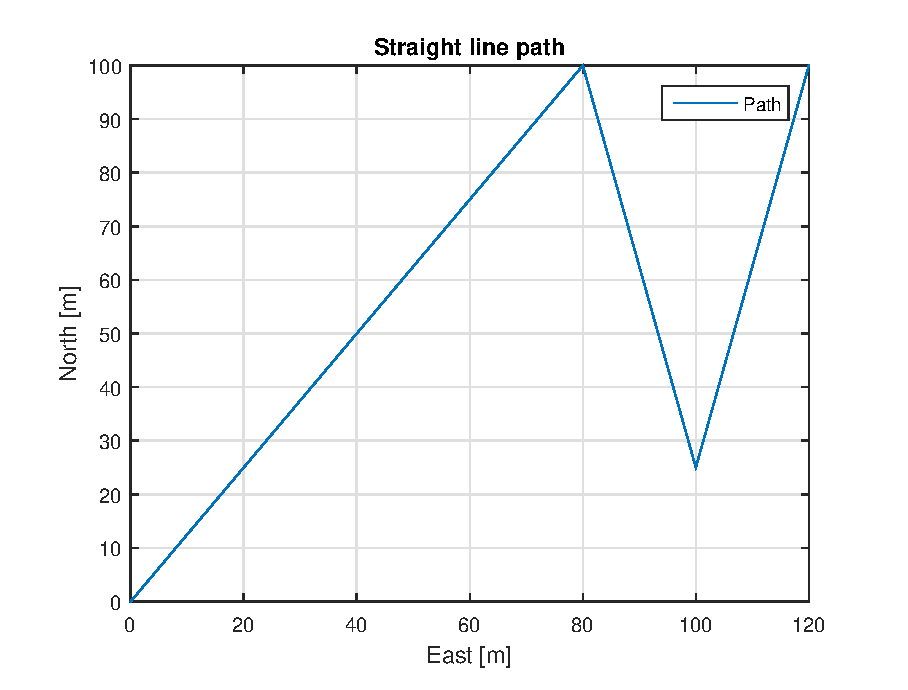
\includegraphics[width=0.7\textwidth]{figs/TheoryPlot/StraightLine.eps}
\end{figure}
The simplest for of creating a path is a straight line between two way-points. The advantage with a straight line is that it's easy for a guidance system to follow the line, however it will experience a jump in reference when transitioning to another straight line due to discontinuous tangential vector.
\section{Dubins path}\label{S:DubinsPath}
An alternative to a straight line path is a path constructed by straight lines and circle. Rudolf Dubin showed \citep{dubins1957curves} that the shortest possible path for a particle that moved with unit speed with maximum curvature would consist of three pieces. The path is considered as the shortest path from $P_s$ to $P_f$, however the curvature is discontinues, which gives a smoothness level of $G^1$ and $C^0$. 
Dubins path is the shortest path from from one way-point to the other which is continues. Dubins path can be created for a three dimensional case, however a simplification is made in which only a planar version of the Dubins path is examined. A Dubin path with fixed end orientation can be constructed in four different way.
\begin{table}[H]
\centering
\begin{adjustbox}{max width=\textwidth}
\begin{tabular}{ | l |}
\hline
Right to Right \\
Right to left \\
Left to Right \\
Left to left \\ \hline
\end{tabular}
\end{adjustbox}
\caption{Turning direction for Dubins path with fixed final orientation}
\label{Tb:DubinsTurningDirection}
\end{table}

Allowing the finish orientation to be free will add four more variants of the Dubins path.
The path consist of two arcs and a straight line. The straight line is tangential to both arcs. The start and end point of the straight line can be found with
\begin{subequations}
\begin{align}
& \alpha = \arcsin\big(\frac{\rho_f-\rho_s}{|c|}\big) \\
& \beta = \arctan\big(\frac{y_{cf}-y_{cs}}{x_{cf}-x_{cs}}\big)
\end{align}
\end{subequations}

\begin{table}[H]
\begin{center}
\begin{tabular}{ | l | | l |}
\hline
& \textbf{Turn angle} \\ \hline
$\phi_{right}$ & $\alpha + \beta + \frac{\pi}{2}$ \\
$\phi_{left}$ & $\beta - \alpha + \frac{3\pi}{2}$ \\ \hline
\end{tabular}
\end{center}
\end{table}

\begin{subequations}
\begin{align}
& x_{P_\chi} = x_{cs} + R_s\cos(\phi) \\
& y_{P_\chi} = x_{cs} + R_s\sin(\phi) \\
& x_{P_N} = x_{cf} + R_f\cos(\phi) \\
& y_{P_N} = x_{cf} + R_f\sin(\phi)
\end{align}
\end{subequations}
\begin{figure}[H]
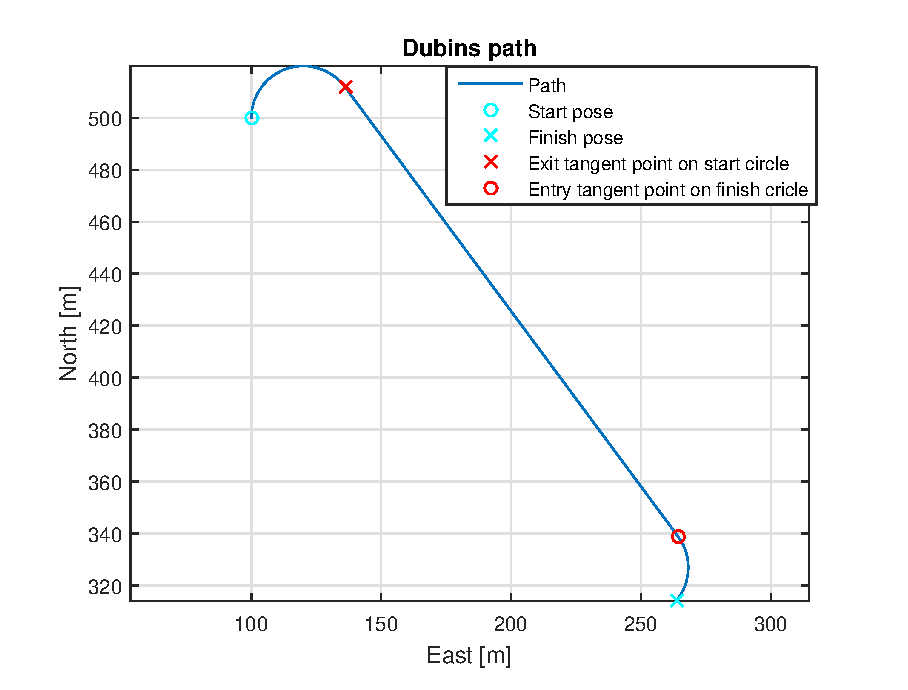
\includegraphics[width=0.7\textwidth]{figs/TheoryPlot/DubinsPath.eps}
\end{figure}
\chapter{RTKGPS}
This chapter present some of the basic theory behind rtkgps.

When phase measurement is applied an important part. Integer ambiguity is the uncertainty of the number of whole cycles between the receiver and a satellite.


\section{Real time kinematic GPS}\label{ss:rtk-gps}
In \citep{misra2011global} section 7.2.2 \arcfull{rtk-gps} is defined as a rover that receive raw measurements from a reference receiver which is transmitted over a radio link, with a key feature that the rover is able to estimate the integer ambiguities while moving. The reference receiver is usually defined as a base station, and the integer ambiguity is the uncertainty of the number of whole phase cycles between the receiver and a satellite. With the measurements from the base station the rover is able to calculated the distance between itself and the base station, where the distance is referred to as a baseline. The length of the baseline affect the accuracy of the \gls{rtk-gps} solution, due to increased effect of atmospheric disturbance, which is further explain in \ref{Ss:Atmosphere}. However with a short baseline, e.g. $1-2 km$, the atmospheric condition can be considered equal for the base station and the rover, which keeps the solution  at centimetre level accuracy.

The ability for the rover to resolve the integer ambiguity is a key feature in \gls{rtk-gps}. A well used method was purposed in the article \citep{teunissen1994new} which decorrelate the integer ambiguities such that a efficient computation of the least square estimate can be performed. The search method is further explained in \citep{teunissen1995least}. A estimate of the integer ambiguity with sufficient high degree of certainty is referred to as a FIX solution, otherwise the solution is degraded to FLOAT where the integer ambiguity is allowed to be a decimal or a floating point number. When the solution is categorised as FIX the accuracy of the solution is considered on centimetre level, while with a FLOAT solution the accuracy is at a decimetre level.

\gls{rtk-gps} can either provide a kinematic setting or a moving baseline setting. The difference between the two is that in kinematic the base station has a known stationary position, while in moving baseline the base station position is unknown and allowed to move. The unknown base station position is calculated with a single receiver, with the accuracy that entails. Therefore the \gls{rtk-gps} system with a moving baseline configuration can never have better global accuracy then what it will get with a single receiver. The advantage with the moving baseline configuration is that \gls{rtk-gps} can be used to find the relative position between two dynamical system using \gls{gnss} in real time. This will be the case in automatic ship landing system, where the base station is on a ship, thus must be allowed to move. The advantage with kinematic mode is that it can give a more accurate position estimate, where the relative position of the rover can be given in either the \gls{ned} or \gls{enu} frame.

\begin{figure}[H]
	\centering
		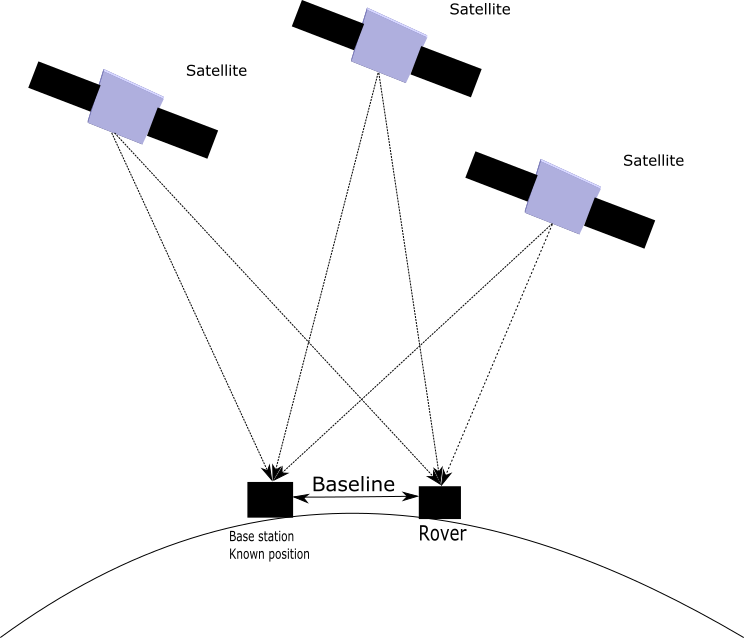
\includegraphics[width=0.7\textwidth]{figs/DGPS.png}
		\caption{Concept figure of \acrfull{dgps}}
		\label{figure:DGPS}
\end{figure}
\section{Error sources}
In order to get high accuracy in the position estimation the different error sources must be identified and removed if possible. This section will identify some of the most significant error sources that can affect the \gls{gnss} signal, and how to remove or mitigate them in the estimation.
\subsection{Clock error}
There is drift in both the satellite clock and the receiver clock. The atomic clock in the satellites makes the clock drift negligible from the user perspective. The receiver clock tend to drift, and if not taken into account will cause large deviations in the position estimate from the true position. This error is remove by including a fourth satellite in the position computation. The satellite clock error is given in the satellite message. 

\subsection{Ionospheric and tropospheric delays}\label{Ss:Atmosphere}
When the \gls{gps} signals travel though the atmosphere there will be a delay caused by the different atmospheric layers.
\subsubsection{Ionospheric delay}
Gas molecules in the ionosphere becomes ionized by the ultraviolet rays that is emitted by the sun, which release free electrons. These electron can influence electromagnetic wave propagation, such as \gls{gnss} signals. In \citep{vik2014integrated} section 3.5.1 it's stated that the delay caused by the ionosphere usually is in the order of $1-10 $meters. The error can be mitigated by using a double frequency receiver, or by applying a mathematical model to estimate the delay. Both those methods are with a single receiver, however by including a second receiver the \gls{gnss} solution system can assume that both receiver receive signal in the same epoch, which means that the signals have experienced the same delay.

\subsubsection{Tropospheric delay}
The tropospheric delay is a function of the local temperature, pressure and relative humidity. From \citep{vik2014integrated} section 3.5.1 the delay can vary from $2.4$ meters to $25$ meters depending on the elevation angle of the satellites. The error can be mitigated by applying a mathematical model to estimate the tropospheric delay, or by using a elevation mask can remove all satellites with a elevation angle bellow a certain threshold. Error caused by tropospheric delay can be removed in the same manners as ionospheric delay when using two or more receivers. 
\subsection{Ephemeris errors}
A satellite is not able to perfectly follow a given orbit, therefore there will be a deviation between satellite position given to the receiver and the true position of the satellite. This is called the ephemeris error. The true position of a satellite is monitored and corrected by the owner of the \gls{gnss} constellation, but error between each correction can be expected.
\subsection{Multipath}
One of the primary source of error in in a GNSS receiver is multipath. Multipath happens when the satellite signal is reflected by a nearby surface before if reach the \gls{gnss} antenna. The delay introduced in the signal can make the receiver believe that its position is several meters away form its true position. The easiest way to mitigated multipath is to place the antenna at a location with open skies, and no tall structures nearby.

Multipath error uncorrelated between receivers, thus the local receiver must be able to correct for multipath error locally.
\cleardoublepage
%\include{RTKGNSS}
\chapter{System}
This chapter contain the description for the system used in the autonomous landing system.
\section{Navigation system}
The navigation system used in the autonomous landing system consist of two sensor packages. The first is part of the pixhawk (REF TIL PIXHAWK), and the other is a Ublox Lea M8T \gls{gnss} receiver suplemented with the open source program RtkLib. The system apply RtkLib for more accurate position and velocity estimation through the use of \gls{rtk-gps}. The output from the RTKGPS software contains only the relative position from the base station, and not the position of the base station. Therefore a task was created to send the global base station location to the navigation system, which enable the rest of the system to calculate the global position of the uav.

The base station position is received in the RTKGPS task in DUNE, were it's included in the GpsFixRtk message.

A task in the nest receive the gps position of the base, and the operator can monitor it in neptus. When the operator choose to fix the base station gps position a parameter update is send to the task, which will start to send a gpsfixrtk message to the uav. 

TODO: Create figure that shows the information flow that is used to create the rtkfix message.
\subsection{Navigation source}
The navigation system is able to receive data from two separate sensor system, which is the Pixhawk package and the Ublock \gls{gnss} receiver with RTKLib. The output from RTKLib is only available if the \gls{rtk-gps} solution is fixed. The default configuration is that the position solution is received from the Pixhawk.

\subsection{Base station}
The base station is able to send it's own gps position to the \gls{uav}. The operator can decide when the base station could be considered as fixed.
\subsection{Operator interface}
The operator use the Neptus platform as operational interface during the landing. The console includes information about the position of the uav, as well as the source of the position measurement. The operator can monitor the status of the gps system, including what is accepted by the navigation system. During a autonomous landing the operator must be fully aware of the status of the navigation system, such that an abort due to lost gps fix. This system can be expanded to include other sensors, like a ranging system, IMU, camera ex.
%\subsection{Position correction}%Flytt til resultat
%The highly dynaimcal nature of the uav create a challenge for the navigation system due to the blocking of the gps antenna from the satellite constellation. The problem was reduced by using a gps receiver that has a high performance in satellite tracking, however this does not remove the problem. A float solution from the gps system is valid for some seconds after fix is lost, due to the predictive nature of the Extended Kalman filter in rtklib. However after a seartin amount of time the navigation system swithces over to use the position estimate from the pixhawk, which has a lower accuracy level then the rtk gps system. To increase the accuracy level a offset solution is proposed. By calculating the difference between the fixed rtk gps solution and the position solution from the pixhawk a offset can be found. If the offset can be assumed constant or quasi stationary it can be used to increase to accuracy level for the navigation system enough to allow for completion of critical phases of a manoeuvre. However tests showed that the offset was not constant nor quasi stationary. By applying the offset to the pixhawk position solution the accuracy level will increase, but not enough to allow for execution of critical manoeuvres.
%In order to make the navigation system more robust, some methods was explored. 
\section{Path generation}
The landing plan is design with the assumption that the aerial space in which the uav operates is limited. The limitation can be the range of the uav, regulatory limits or weather. In addition the autonomous landing system must be able to perform a safe landing from any initial position. Furthermore the size of the virtual run way should be constructed by the operator. The type of uav operation dictates the maximum size of the landing path. Different types of uav operation is LOS, ELOS, BLOS and BRLOS. Only the first is considered in this thesis, which means that the pilot must have the uav in view during the entire flight. The operator must also be able to control the angle which the uav is descending, which means that the height of the landing path is fixed. Therefore the uav must be at the correct altitude before it can start descending toward the landing net.

A landing plan that is proposed consist of Dubins path \ref{S:DubinsPath} in the lateral plane, and straight lines in the longitudinal plane. The path is generated from an arbitrary start positing, and will create a continuous path toward the landing approach. The design is inspired by the work done in \citep{Skulstad&Syversen} were way-points was used to guide the uav toward the landing approach.

The plan is generated in a Dune task which receive a plan generation request from Neptus. Then a plan is created, which is sent to the Dune task Plan manager, which in turn sent desired state to the guidance system. The plan is decoupled from the guidance system, which allow for use of different control design when executing the landing plan.

The Dubin path is constructed with a followPath manoeuvre.

The landing plan generated by the Dune task can be requested for review by the operator in Neptus. The plan will not start before the operator has reviewed the plan, and approved by uploading it to the uav. In the uploaded version a specification list on which controller that should be used is included.  
\subsection{The net approach}
The net approach path consist a straight line in the lateral plain, and straight lines in the longitudinal plane. The net approach way-points are defined relative to the position of the net, which has been defined as origo. The four way-points in the net approach is defined as follows:
\begin{subequations}
\begin{align}
&\mathbf{WP1} = 
\begin{bmatrix}
-a0 \\
0 \\
h_{nc} + a1\tan(\gamma_a) 
\end{bmatrix}\\
&\mathbf{WP2} = 
\begin{bmatrix}
a1 \\
0 \\
h_{nc} - a1\tan(\gamma_a)
\end{bmatrix}\\
&\mathbf{WP3} = \mathbf{WP2} + 
\begin{bmatrix}
a2 \\
0 \\
a2\tan(\gamma_d)
\end{bmatrix}\\
&\mathbf{WP4} = \mathbf{WP3} + 
\begin{bmatrix}
a3 \\
0 \\
0 \\
\end{bmatrix}
\end{align}
\end{subequations}
were the description of the parameters used is given in table \ref{Tb:Approach Parameters}. The net is placed between the first and second way points such that transitional behaviour do not occur during the finale stage of the net landing. In addition the path has been made with the assumption that the $\gamma_a$ and $\gamma_d$ is considered small. This assumption is made to easy the demand of the controllers used in the landing system.
\begin{table}[H]
\begin{center}
    \begin{tabular}{ | l | l |}
    \hline
    \textbf{Parameter} & \textbf{Description} \\ \hline
    $a0$ & The distance behind the net \\ \hline
    $a1$ & The distance in front of the net \\ \hline
    $a2$ & The length of the glide slope \\ \hline
    $a3$ & The length of the approach towards the glide slope \\ \hline
    $\gamma_a$ & The net attack angle \\ \hline
    $\gamma_d$ & The glide slope angle \\ \hline
    \end{tabular}
\end{center}
\caption{Net approach parameters }
\label{Tb:Approach Parameters}
\end{table}
The way point vectors are rotated into the NED frame by a rotation around the z-axes.
\begin{equation}
WP^n = R(\psi_{net})WP^b
\end{equation}
were $\psi_{net}$ is the heading of the net.
\begin{figure}
\def\svgwidth{\textwidth} % Defining the width since Inkscape hasn't done this yet in the .pdf_tex file
\input{InkFig/LandingPhase.pdf_tex}
\end{figure}

\subsection{The landing path approach}
In order for the \gls{uav} to be able to start the landing approach the \gls{uav} must be at the correct altitude with the correct orientation from any initial position. That require a path which the \gls{uav} is able to follow. The problem can be separated into two parts. The first is the longitudinal parts, while the other is the lateral. The longitudinal path will be more exposed to large changes in heading, which puts demands of the type of path that can be chosen. However since a time demand is not required the problem becomes a path following problem. The problem has been solved by creating a Dubins path in the longitudinal plane.

A desired behaviour in the lateral plane is that the \gls{uav} should have a controlled decent. Given this desired behaviour it was decided that the lateral plane should be a glide slope, which means that the decent angle can be considered small. The strategy chosen to solve this problem is the use of straight lines in the lateral plane. The straight lines are is included with Dubins path such that the turn in Dubins path becomes a spiral.

At the end of Dubins path the path is checked if the correct height has been reach. If the correct height has not been reached the path will create a spiral that converge to the correct height. When the correct height has been reach a last arc is created in order for the \gls{uav} to get the correct orientation.

The landing path can be created in two modes, which is manual or automatic. The manual mode allow the operator to design the landing path by defined the turning direction for the start and final circle. This enable the operator to specify a path that fills a operational demand, which would not necessary be the path when in automatic.

In automatic mode all four variants, which is given in table \ref{Tb:DubinsTurningDirection}, calculated. After the length of the paths are calculated, where the shortest path is chosen to be the landing path.
The landing path approach can be generated in to different way. One mode allow for manual deciding which side the start and finish circle should be in respect on the start pose, and the net landing approach. This allow the operator full control over the landing path, and can choose a landing path that is operation feasible and not necessary the shortest path. 
\subsubsection{Extra way point}
To ensure that the path generation system will generate å flyable path an extra way point is added in the case of the start pose in cause an infeasable dubins path, or an spesial case of Dubins path which has not been implemented. The two case are
\begin{subequations}
\end{subequations}
\section{Evasion}
To ensure the safety of the operator a evasion controller is used to abort the landing when a successful landing is deemed infeasible or improbable.

\section{Guidance system}
The guidance system consist of two part. Sliding mode controller, and a los controller

\subsection{Sliding mode controller}
For course control the system use a sliding mode controller that was proposed in the paper \citep{fortuna2015cascaded}, which USGES stability property.
\begin{subequations}
\begin{align}
\dot{x} &= V_a\cos(\psi) + W_x = V_g\cos(\psi) \\
\dot{y} &= V_a\sin(\psi) + W_y = V_g\sin(\psi) \\
\dot{phi} &= \frac{g}{V_a}\tan(\varphi) \\
\dot{\varphi} &= -\frac{\varphi-\varphi_{cmd}}{T_\varphi} \\
W &= \sqrt{W_x^2 + W_y^2}
\end{align}
\end{subequations}
\begin{equation}
\epsilon(\varphi) = \begin{cases}
\cos(\varphi), & \text{if}\ |\cos(\varphi)|\geq\epsilon'\\
\epsilon', & \text{if}\ 0 \leq \cos(\varphi) < \epsilon' \\
-\epsilon', & \text{if} -\epsilon'<\cos(\varphi) < 0
\end{cases}
\end{equation}
\begin{equation}
\chi = \tan^{-1}(\frac{\dot{y}}{\dot{x}})
\end{equation}
\begin{equation}
\dot{\chi} = \frac{g\sin(\varphi)(V_a + \cos(\psi)W_x + \sin(\psi)W_y}{\epsilon(\varphi)V_g^2}
\end{equation}
\begin{subequations}
\begin{align}
\chi_d &= \tan^{-1}(-\frac{t}{\Delta} \\
\dot{\chi_d} &= -\frac{\Delta}{\Delta^2+y^2}\dot{y} \\
\ddot{\chi} &= \frac{\Delta}{(\Delta^2 + y^2)^2}(2y\dot{y}^2 - (\Delta^2 + y^2)\ddot{y})
\end{align}
\end{subequations}
\begin{equation}
\tilde{\chi} = \chi - \chi_d
\end{equation}
\begin{equation}
s = \dot{\tilde{\chi}} + \lambda\tilde{\chi}
\end{equation}
\begin{equation}
u = -\lambda\dot{\tilde{\chi}} - \rho\text{sgn}(s) - K_ds
\end{equation}
%\chapter{Implementation}
This chapter contain the technical specification of the navigation system and landing path system, in addition to the payload installed in the X8 and both nests.
\begin{figure}[H]
	\centering
		\includegraphics[width=1\textwidth]{figs/DUNESystem.png}
		\caption{A simplified figure of the Dune auto land system}
		\label{figure:RTKLIB_STRUCTURE}
\end{figure}
\section{Landing path}
The landing path is specified through the Neptus plug-in LandmapLayer, which allow for real time setting of the parameters used to create the landing path. In addition the plug-in display the position of the net in the graphical map interface which is a part of Neptus. The plug-in dispatch the \gls{imc} message, LandingPlanGeneration, which has been created specifically for landing path purpose.

The \gls{imc} LandingPlanGeneration message is dispatch to the Dune system, where it's picked up by the Dune task LandingPlan. This trigger the generation of the landing path, and depending on the configuration of the Dune task and desired setting in the LandingPlanGeneration message different landing path is generated. The different variants is categorised into two groups; configuration of the Dubins path, and configuration of the virtual runway. The configuration option that result in different variants of the landing path is given in table \ref{Tb:DubinConfig}. In addition the Dune task can be configured for a dynamical landing. When configured as dynamical it's assumed that an other task is responsible for the final landing part. Therefore the vertical runway is not part of the plan, however the first part of the path is still included.
\begin{table}
\centering
\begin{tabular}{| p{2.7cm} | | p{6cm} |}
\hline
\textbf{Parameter name} 							& \textbf{Action} \\ \hline
 Automatic (boolean)								& If true a standard path where the shortest Dubins path is chosen. Otherwise a user specific path is chosen \\ \hline
Start circle turning counter clockwise (boolean)	& If true the start arc is created such that the turning direction is counter clockwise. Otherwise clockwise. Require Automatic==false \\ \hline
Finish circle turning counter clockwise (boolean)	& If true the finish arc is created such that the turning direction is counter clockwise. Otherwise clockwise. Require Automatic==false \\ \hline
Wait at loiter (boolean)							& If true a unlimited loiter is included in the path before the path continue with the path along the virtual runway. \\ \hline

\end{tabular}
\label{Tb:DubinConfig}
\end{table}

A design choice allows for user determined rotation direction. By setting the "automatic" flag to false in the \gls{imc} message LandingPlanGeneration the rotation direction is determined by the flags "startCounterClockwise" and "finishCounterClockwise".


When generated the plan must be started from Neptus, where the desired control configuration is added to the path.

A loiter manoeuvre can be included in the landing plan before the start of the path along the virtual runway. The loiter manoeuvre can be used to control when the \gls{uav} should start it's final approach, which is practical when performing a dynamical landing.
\section{Navigation system}
The navigation system is control by a state machine \ref{S:NavState}, which is used to control the content of the output \gls{imc} messages EstimatedState and NavSources. Depending on which state the navigation system is in the \gls{imc} EstimatedState message will either have position solution form the \gls{rtk-gps} system or the external navigation system. During a short loss of the RTK the external navigation position is compensated with the average difference between the RTK solution and the external navigation solution.
\subsection{RTK-GPS system}
The \gls{rtk-gps} solution is dispatched from the DUNE task RTKGPS, however before the message is accepted by the Navigation task the message must include a valid base station position. The base station position is not included in the output message from RTKlib, which demand the base station position to be calculated locally at the base station as a standalone \gls{gnss} receiver. For this purpose the DUNE task BasestationFix is used to lock the current position of the base station, which result in the base station position being transmitted to the RTKGPS task.
The navigation system require to now the reference position of the base station in order to use the \gls{rtk-gps} solution. However the base station position is currently not part of the output message from rtkrcv. This is resolved by allowing the base station to calculate it's own position as a standalone \gls{gps}. The \gls{gps} position is transmitted to a local Dune task on the base station, where the operator can decide when the base station can be considered as fixed. When the base station is considered fixed the position is sent to the X8, where it's included in the \gls{rtk-gps} solution message.
\subsubsection{Nest system}
A nest system is a stationary unit with the sole purpose of providing it's position to the rest of the Dune System. As part of the navigation system the base station is defined as a nest, where the \gls{gps} position is sent to the \gls{rtk-gps} system when fixed.
An other nest has been created to obtain the \gls{gps} position of the stationary net. The net nest is configured as a rover in \gls{rtk-gps} configuration, such that the position relative to the base station is in the same frame as the X8.
\subsection{Operator interface}
The state of the navigation system is monitored though a interface in Neptus. The interface indicate which source the Dune system is using for state information. The interfaced apply a color code to indicate which source is currently in use in addition to all sensor system that are available, as seen in table \ref{Tb:Color Code}.
\begin{table}[H]
\begin{center}
    \begin{tabular}{ | l | l |}
    \hline
    \textbf{Color} & \textbf{Description} \\ \hline
    White & Not available \\ \hline
    Yellow & Available, but not in use \\ \hline
    Green & Available, and in use \\ \hline
    \end{tabular}
\end{center}
\caption{Net approach parameters }
\label{Tb:Color Code}
\end{table}
%\chapter{Experiment}
\section{Path}
\subsection{Landing path with pixhawk autopilot}
A landing path was create with the goal of testing the concept of the landing path system. The test was perform with the pixhawk autopilot, and navigation system. Thus high performance from the X8 is not expected. The path was create in cooperation with the operator and pilot, which dictated the maximum size of the landing path.

The height where the \gls{uav} held after the approach path was to low, and during a real landing would cause the \gls{uav} to crash. Thus either the length of the landing path or the glide slope angle has to increase. The performance of the pixhawk autopilot was not adequate to successfully hit the net.

The wind condition was measured to be $5m/s$ from the north, which caused the \gls{uav} to have to perform the landing with a cross wind.

The path was created with manually deciding the rotation directions, due to the start position and where the operator wanted the \gls{uav} to circle down to the correct height. In this case the shortest path would bring the \gls{uav} close to a no-fly zone


\begin{figure}[H]
	\centering
		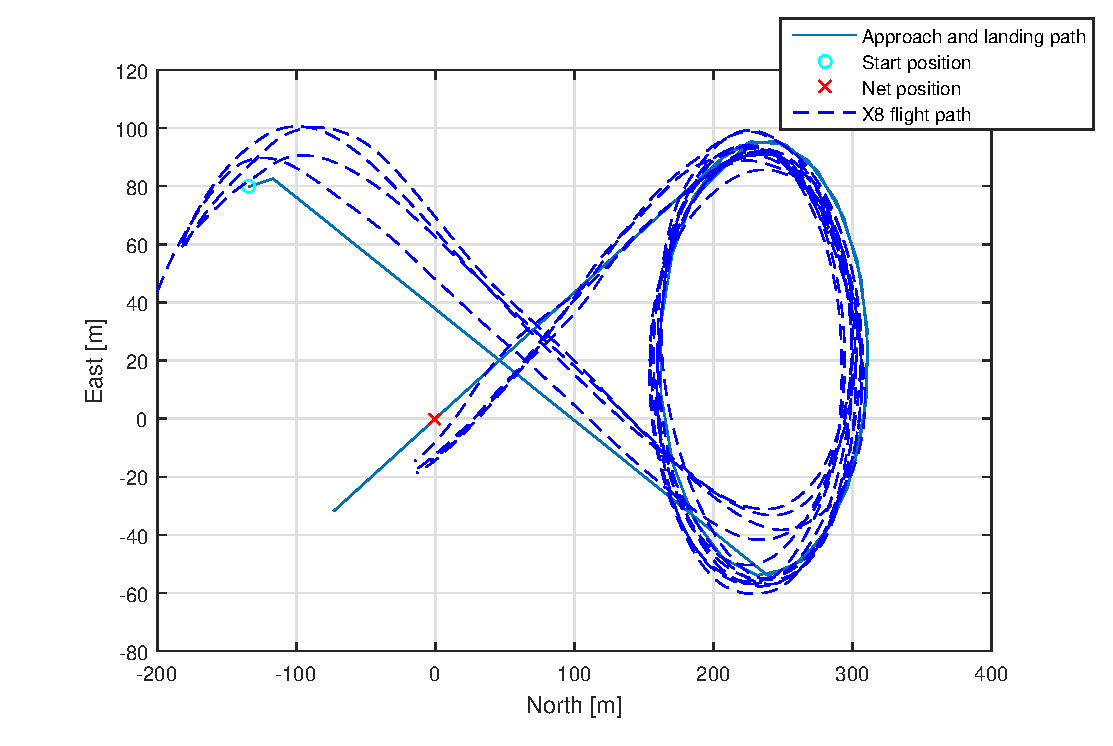
\includegraphics[width=1\textwidth]{figs/Experiment/NorthEastLandingPathArdu.eps}
		\caption{Four lateral flight paths towards the net position}
		\label{Fig:NorthEastArdu}
\end{figure}
\section{Navigation}
The navigation system was tested in both a X8 and in a multicopter system.

\subsection{Formation position}
The accuracy of the \gls{rtk-gps} position system was tested with two mutlicopter system, with the goal of measuring the distance between them. During stationary conditions it was determined that \gls{rtk-gps} was highly accurate, and is required when performing a formation flight. The same principle is used in determining the net position, where the net nest apply \gls{rtk-gps} to determine it's own position. However currently the position has to manually be written to Neptus, which must change when performing a ship landing.
\subsection{Short loss compensator}
Include result when short loss was not in use. Compare to result when it's in use.

The short loss compensator bring the position solution from the pixhawk close enough to the \gls{rtk-gps} solution such that the navigation system does not lose its position. However a highly aggressive control system that attempt to keep the error at centimeter level is expected to react to the discontinues introduced from the compensator. All though currently it has not been concluded that the compensator cause problems for the control system, since failure has happen during demanding wind condition. 
%\include{Discusion}
%% include here the other chapters

\renewcommand*{\bibname}{References}
\bibliographystyle{plainnat}
\bibliography{main}

%% Uncomment the following if you have any appendix
 \appendix
 \addtocontents{toc}{%
  \protect\vspace{1em}% 
  \protect\noindent \bfseries \appendixtocname\protect\par
  \protect\vspace{-.5em}%
 }
 \renewcommand{\chaptername}{\appendixname}
%% include below possible appendices (chapters)
\chapter{Rtklib Configuration}\label{APPENDIX:RTKLIB}
This appendix chapter contain the configuration file used to configure RTKlib in the X8, which is given as:
\verbatiminput{rtkrcv.conf}

\end{document} 
